\documentclass[tikz, border=6pt]{standalone}
\IfFileExists{lmodern.sty}{\usepackage[T1]{fontenc}\usepackage{lmodern}}{}
\usepackage{amsmath,amssymb,bm}
\usepackage[scaled=0.95]{helvet}
\usetikzlibrary{arrows.meta, decorations.pathreplacing}
\definecolor{Green}{HTML}{3BA55C}
\definecolor{Orange}{HTML}{EE8133}
\definecolor{Red}{HTML}{DF4B4B}
\definecolor{Purple}{HTML}{8459D1}
\definecolor{Gray}{HTML}{6B7280}
\definecolor{Ink}{HTML}{1F2937}
\colorlet{input}{Green}
\colorlet{conv}{Orange}
\colorlet{pool}{Red}
\colorlet{softmax}{Green}
\begin{document}
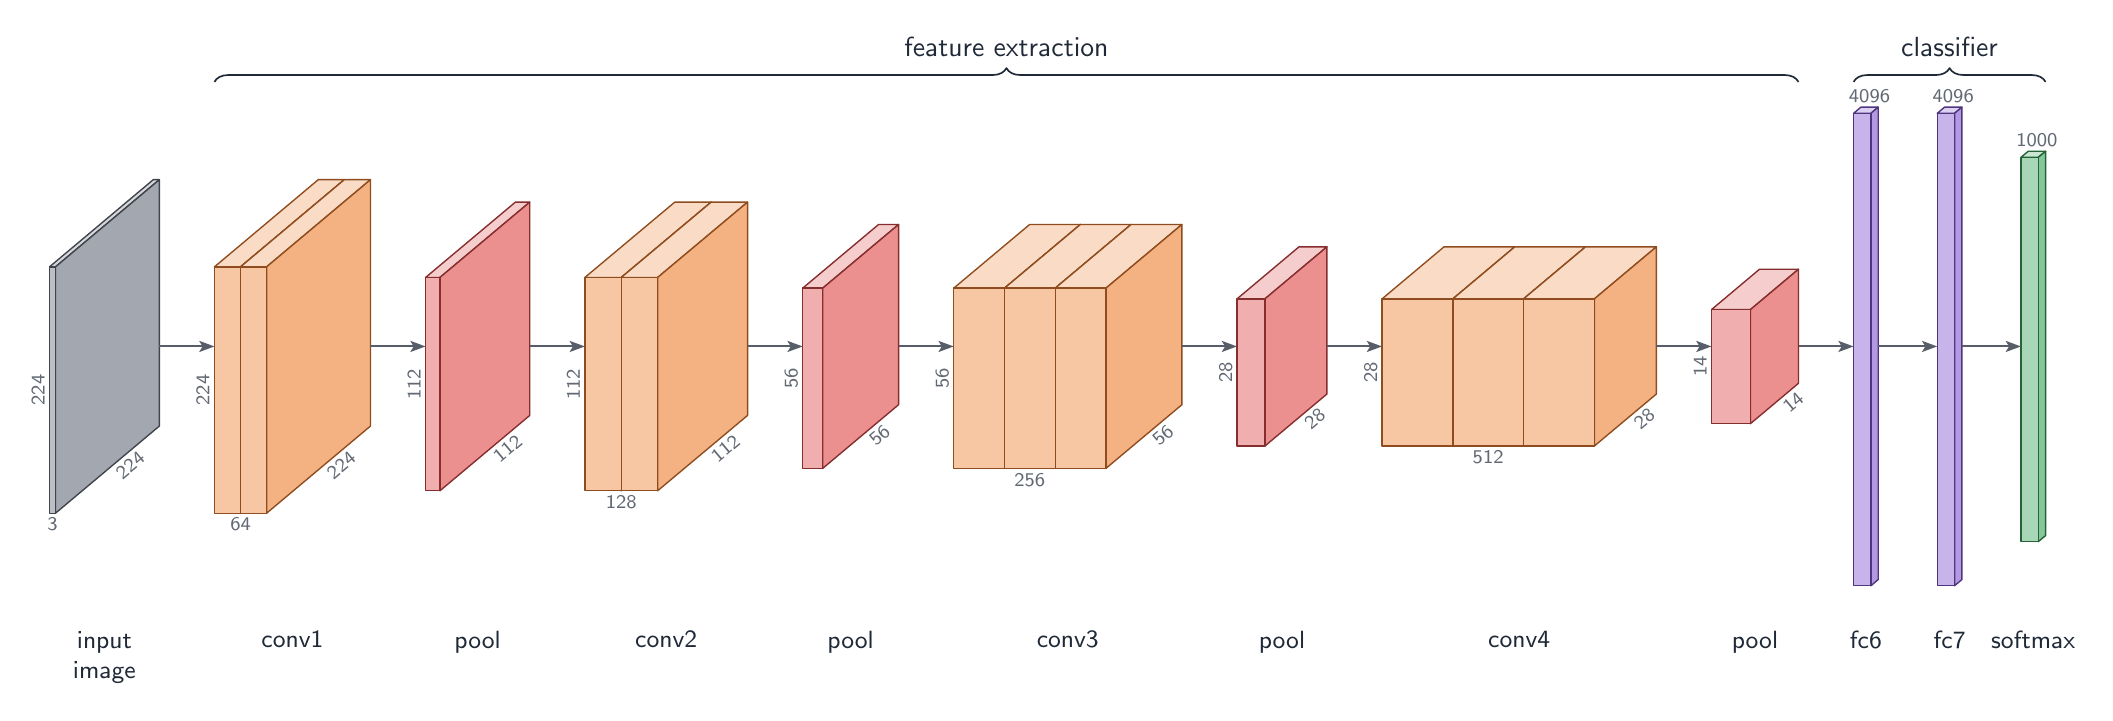
\begin{tikzpicture}[color=Ink, execute at begin picture={\sffamily}, line width=0.6pt, >={Stealth[length=5.5pt, width=4pt, inset=1.2pt]}, line join=round]
  % conv net cnn
  % block 0: input
image
  \filldraw[fill=Gray!28, draw=Gray!60!black, line width=0.5pt] (0,1.011) -- (0.076,1.011) -- (1.395,2.118) -- (1.318,2.118) -- cycle;
  \filldraw[fill=Gray!62, draw=Gray!60!black, line width=0.5pt] (0.076,-2.118) -- (1.395,-1.011) -- (1.395,2.118) -- (0.076,1.011) -- cycle;
  \filldraw[fill=Gray!45, draw=Gray!60!black, line width=0.5pt] (0,-2.118) rectangle (0.076,1.011);
  \node[anchor=south, rotate=90, font=\scriptsize, text=Ink!70, inner sep=1.5pt] at (0,-0.553) {224};
  \node[anchor=north west, rotate=40, font=\scriptsize, text=Ink!70, inner sep=1.5pt] at (0.735,-1.565) {224};
  \node[anchor=north, font=\scriptsize, text=Ink!70, inner sep=1.5pt] at (0.038,-2.118) {3};
  % block 1: conv1
  \filldraw[fill=Orange!28, draw=Orange!60!black, line width=0.5pt] (2.095,1.011) -- (2.426,1.011) -- (3.744,2.118) -- (3.413,2.118) -- cycle;
  \filldraw[fill=Orange!62, draw=Orange!60!black, line width=0.5pt] (2.426,-2.118) -- (3.744,-1.011) -- (3.744,2.118) -- (2.426,1.011) -- cycle;
  \filldraw[fill=Orange!45, draw=Orange!60!black, line width=0.5pt] (2.095,-2.118) rectangle (2.426,1.011);
  \filldraw[fill=Orange!28, draw=Orange!60!black, line width=0.5pt] (2.426,1.011) -- (2.757,1.011) -- (4.076,2.118) -- (3.744,2.118) -- cycle;
  \filldraw[fill=Orange!62, draw=Orange!60!black, line width=0.5pt] (2.757,-2.118) -- (4.076,-1.011) -- (4.076,2.118) -- (2.757,1.011) -- cycle;
  \filldraw[fill=Orange!45, draw=Orange!60!black, line width=0.5pt] (2.426,-2.118) rectangle (2.757,1.011);
  \node[anchor=south, rotate=90, font=\scriptsize, text=Ink!70, inner sep=1.5pt] at (2.095,-0.553) {224};
  \node[anchor=north west, rotate=40, font=\scriptsize, text=Ink!70, inner sep=1.5pt] at (3.416,-1.565) {224};
  \node[anchor=north, font=\scriptsize, text=Ink!70, inner sep=1.5pt] at (2.426,-2.118) {64};
  % block 2: pool
  \filldraw[fill=Red!28, draw=Red!60!black, line width=0.5pt] (4.776,0.876) -- (4.958,0.876) -- (6.099,1.833) -- (5.917,1.833) -- cycle;
  \filldraw[fill=Red!62, draw=Red!60!black, line width=0.5pt] (4.958,-1.833) -- (6.099,-0.876) -- (6.099,1.833) -- (4.958,0.876) -- cycle;
  \filldraw[fill=Red!45, draw=Red!60!black, line width=0.5pt] (4.776,-1.833) rectangle (4.958,0.876);
  \node[anchor=south, rotate=90, font=\scriptsize, text=Ink!70, inner sep=1.5pt] at (4.776,-0.479) {112};
  \node[anchor=north west, rotate=40, font=\scriptsize, text=Ink!70, inner sep=1.5pt] at (5.528,-1.355) {112};
  % block 3: conv2
  \filldraw[fill=Orange!28, draw=Orange!60!black, line width=0.5pt] (6.799,0.876) -- (7.261,0.876) -- (8.403,1.833) -- (7.941,1.833) -- cycle;
  \filldraw[fill=Orange!62, draw=Orange!60!black, line width=0.5pt] (7.261,-1.833) -- (8.403,-0.876) -- (8.403,1.833) -- (7.261,0.876) -- cycle;
  \filldraw[fill=Orange!45, draw=Orange!60!black, line width=0.5pt] (6.799,-1.833) rectangle (7.261,0.876);
  \filldraw[fill=Orange!28, draw=Orange!60!black, line width=0.5pt] (7.261,0.876) -- (7.723,0.876) -- (8.865,1.833) -- (8.403,1.833) -- cycle;
  \filldraw[fill=Orange!62, draw=Orange!60!black, line width=0.5pt] (7.723,-1.833) -- (8.865,-0.876) -- (8.865,1.833) -- (7.723,0.876) -- cycle;
  \filldraw[fill=Orange!45, draw=Orange!60!black, line width=0.5pt] (7.261,-1.833) rectangle (7.723,0.876);
  \node[anchor=south, rotate=90, font=\scriptsize, text=Ink!70, inner sep=1.5pt] at (6.799,-0.479) {112};
  \node[anchor=north west, rotate=40, font=\scriptsize, text=Ink!70, inner sep=1.5pt] at (8.294,-1.355) {112};
  \node[anchor=north, font=\scriptsize, text=Ink!70, inner sep=1.5pt] at (7.261,-1.833) {128};
  % block 4: pool
  \filldraw[fill=Red!28, draw=Red!60!black, line width=0.5pt] (9.565,0.74) -- (9.819,0.74) -- (10.783,1.549) -- (10.529,1.549) -- cycle;
  \filldraw[fill=Red!62, draw=Red!60!black, line width=0.5pt] (9.819,-1.549) -- (10.783,-0.74) -- (10.783,1.549) -- (9.819,0.74) -- cycle;
  \filldraw[fill=Red!45, draw=Red!60!black, line width=0.5pt] (9.565,-1.549) rectangle (9.819,0.74);
  \node[anchor=south, rotate=90, font=\scriptsize, text=Ink!70, inner sep=1.5pt] at (9.565,-0.405) {56};
  \node[anchor=north west, rotate=40, font=\scriptsize, text=Ink!70, inner sep=1.5pt] at (10.301,-1.145) {56};
  % block 5: conv3
  \filldraw[fill=Orange!28, draw=Orange!60!black, line width=0.5pt] (11.483,0.74) -- (12.128,0.74) -- (13.092,1.549) -- (12.448,1.549) -- cycle;
  \filldraw[fill=Orange!62, draw=Orange!60!black, line width=0.5pt] (12.128,-1.549) -- (13.092,-0.74) -- (13.092,1.549) -- (12.128,0.74) -- cycle;
  \filldraw[fill=Orange!45, draw=Orange!60!black, line width=0.5pt] (11.483,-1.549) rectangle (12.128,0.74);
  \filldraw[fill=Orange!28, draw=Orange!60!black, line width=0.5pt] (12.128,0.74) -- (12.772,0.74) -- (13.736,1.549) -- (13.092,1.549) -- cycle;
  \filldraw[fill=Orange!62, draw=Orange!60!black, line width=0.5pt] (12.772,-1.549) -- (13.736,-0.74) -- (13.736,1.549) -- (12.772,0.74) -- cycle;
  \filldraw[fill=Orange!45, draw=Orange!60!black, line width=0.5pt] (12.128,-1.549) rectangle (12.772,0.74);
  \filldraw[fill=Orange!28, draw=Orange!60!black, line width=0.5pt] (12.772,0.74) -- (13.416,0.74) -- (14.381,1.549) -- (13.736,1.549) -- cycle;
  \filldraw[fill=Orange!62, draw=Orange!60!black, line width=0.5pt] (13.416,-1.549) -- (14.381,-0.74) -- (14.381,1.549) -- (13.416,0.74) -- cycle;
  \filldraw[fill=Orange!45, draw=Orange!60!black, line width=0.5pt] (12.772,-1.549) rectangle (13.416,0.74);
  \node[anchor=south, rotate=90, font=\scriptsize, text=Ink!70, inner sep=1.5pt] at (11.483,-0.405) {56};
  \node[anchor=north west, rotate=40, font=\scriptsize, text=Ink!70, inner sep=1.5pt] at (13.899,-1.145) {56};
  \node[anchor=north, font=\scriptsize, text=Ink!70, inner sep=1.5pt] at (12.45,-1.549) {256};
  % block 6: pool
  \filldraw[fill=Red!28, draw=Red!60!black, line width=0.5pt] (15.081,0.604) -- (15.435,0.604) -- (16.223,1.265) -- (15.868,1.265) -- cycle;
  \filldraw[fill=Red!62, draw=Red!60!black, line width=0.5pt] (15.435,-1.265) -- (16.223,-0.604) -- (16.223,1.265) -- (15.435,0.604) -- cycle;
  \filldraw[fill=Red!45, draw=Red!60!black, line width=0.5pt] (15.081,-1.265) rectangle (15.435,0.604);
  \node[anchor=south, rotate=90, font=\scriptsize, text=Ink!70, inner sep=1.5pt] at (15.081,-0.33) {28};
  \node[anchor=north west, rotate=40, font=\scriptsize, text=Ink!70, inner sep=1.5pt] at (15.829,-0.935) {28};
  % block 7: conv4
  \filldraw[fill=Orange!28, draw=Orange!60!black, line width=0.5pt] (16.923,0.604) -- (17.822,0.604) -- (18.609,1.265) -- (17.71,1.265) -- cycle;
  \filldraw[fill=Orange!62, draw=Orange!60!black, line width=0.5pt] (17.822,-1.265) -- (18.609,-0.604) -- (18.609,1.265) -- (17.822,0.604) -- cycle;
  \filldraw[fill=Orange!45, draw=Orange!60!black, line width=0.5pt] (16.923,-1.265) rectangle (17.822,0.604);
  \filldraw[fill=Orange!28, draw=Orange!60!black, line width=0.5pt] (17.822,0.604) -- (18.72,0.604) -- (19.508,1.265) -- (18.609,1.265) -- cycle;
  \filldraw[fill=Orange!62, draw=Orange!60!black, line width=0.5pt] (18.72,-1.265) -- (19.508,-0.604) -- (19.508,1.265) -- (18.72,0.604) -- cycle;
  \filldraw[fill=Orange!45, draw=Orange!60!black, line width=0.5pt] (17.822,-1.265) rectangle (18.72,0.604);
  \filldraw[fill=Orange!28, draw=Orange!60!black, line width=0.5pt] (18.72,0.604) -- (19.619,0.604) -- (20.407,1.265) -- (19.508,1.265) -- cycle;
  \filldraw[fill=Orange!62, draw=Orange!60!black, line width=0.5pt] (19.619,-1.265) -- (20.407,-0.604) -- (20.407,1.265) -- (19.619,0.604) -- cycle;
  \filldraw[fill=Orange!45, draw=Orange!60!black, line width=0.5pt] (18.72,-1.265) rectangle (19.619,0.604);
  \node[anchor=south, rotate=90, font=\scriptsize, text=Ink!70, inner sep=1.5pt] at (16.923,-0.33) {28};
  \node[anchor=north west, rotate=40, font=\scriptsize, text=Ink!70, inner sep=1.5pt] at (20.013,-0.935) {28};
  \node[anchor=north, font=\scriptsize, text=Ink!70, inner sep=1.5pt] at (18.271,-1.265) {512};
  % block 8: pool
  \filldraw[fill=Red!28, draw=Red!60!black, line width=0.5pt] (21.107,0.468) -- (21.601,0.468) -- (22.212,0.981) -- (21.717,0.981) -- cycle;
  \filldraw[fill=Red!62, draw=Red!60!black, line width=0.5pt] (21.601,-0.981) -- (22.212,-0.468) -- (22.212,0.981) -- (21.601,0.468) -- cycle;
  \filldraw[fill=Red!45, draw=Red!60!black, line width=0.5pt] (21.107,-0.981) rectangle (21.601,0.468);
  \node[anchor=south, rotate=90, font=\scriptsize, text=Ink!70, inner sep=1.5pt] at (21.107,-0.256) {14};
  \node[anchor=north west, rotate=40, font=\scriptsize, text=Ink!70, inner sep=1.5pt] at (21.906,-0.725) {14};
  % block 9: fc6
  \filldraw[fill=Purple!28, draw=Purple!60!black, line width=0.5pt] (22.912,2.961) -- (23.132,2.961) -- (23.224,3.039) -- (23.004,3.039) -- cycle;
  \filldraw[fill=Purple!62, draw=Purple!60!black, line width=0.5pt] (23.132,-3.039) -- (23.224,-2.961) -- (23.224,3.039) -- (23.132,2.961) -- cycle;
  \filldraw[fill=Purple!45, draw=Purple!60!black, line width=0.5pt] (22.912,-3.039) rectangle (23.132,2.961);
  \node[anchor=south, font=\scriptsize, text=Ink!70, inner sep=1.5pt] at (23.114,3.039) {4096};
  % block 10: fc7
  \filldraw[fill=Purple!28, draw=Purple!60!black, line width=0.5pt] (23.974,2.961) -- (24.194,2.961) -- (24.287,3.039) -- (24.067,3.039) -- cycle;
  \filldraw[fill=Purple!62, draw=Purple!60!black, line width=0.5pt] (24.194,-3.039) -- (24.287,-2.961) -- (24.287,3.039) -- (24.194,2.961) -- cycle;
  \filldraw[fill=Purple!45, draw=Purple!60!black, line width=0.5pt] (23.974,-3.039) rectangle (24.194,2.961);
  \node[anchor=south, font=\scriptsize, text=Ink!70, inner sep=1.5pt] at (24.177,3.039) {4096};
  % block 11: softmax
  \filldraw[fill=Green!28, draw=Green!60!black, line width=0.5pt] (25.037,2.402) -- (25.257,2.402) -- (25.35,2.479) -- (25.13,2.479) -- cycle;
  \filldraw[fill=Green!62, draw=Green!60!black, line width=0.5pt] (25.257,-2.479) -- (25.35,-2.402) -- (25.35,2.479) -- (25.257,2.402) -- cycle;
  \filldraw[fill=Green!45, draw=Green!60!black, line width=0.5pt] (25.037,-2.479) rectangle (25.257,2.402);
  \node[anchor=south, font=\scriptsize, text=Ink!70, inner sep=1.5pt] at (25.24,2.479) {1000};
  \draw[->, Ink!75, line width=0.7pt] (1.395,0) -- (2.095,0);
  \draw[->, Ink!75, line width=0.7pt] (4.076,0) -- (4.776,0);
  \draw[->, Ink!75, line width=0.7pt] (6.099,0) -- (6.799,0);
  \draw[->, Ink!75, line width=0.7pt] (8.865,0) -- (9.565,0);
  \draw[->, Ink!75, line width=0.7pt] (10.783,0) -- (11.483,0);
  \draw[->, Ink!75, line width=0.7pt] (14.381,0) -- (15.081,0);
  \draw[->, Ink!75, line width=0.7pt] (16.223,0) -- (16.923,0);
  \draw[->, Ink!75, line width=0.7pt] (20.407,0) -- (21.107,0);
  \draw[->, Ink!75, line width=0.7pt] (22.212,0) -- (22.912,0);
  \draw[->, Ink!75, line width=0.7pt] (23.224,0) -- (23.974,0);
  \draw[->, Ink!75, line width=0.7pt] (24.287,0) -- (25.037,0);
  \node[anchor=north, font=\small, align=center] at (0.697,-3.489) {input\\image};
  \node[anchor=north, font=\small, align=center] at (3.085,-3.489) {conv1};
  \node[anchor=north, font=\small, align=center] at (5.437,-3.489) {pool};
  \node[anchor=north, font=\small, align=center] at (7.832,-3.489) {conv2};
  \node[anchor=north, font=\small, align=center] at (10.174,-3.489) {pool};
  \node[anchor=north, font=\small, align=center] at (12.932,-3.489) {conv3};
  \node[anchor=north, font=\small, align=center] at (15.652,-3.489) {pool};
  \node[anchor=north, font=\small, align=center] at (18.665,-3.489) {conv4};
  \node[anchor=north, font=\small, align=center] at (21.659,-3.489) {pool};
  \node[anchor=north, font=\small, align=center] at (23.068,-3.489) {fc6};
  \node[anchor=north, font=\small, align=center] at (24.131,-3.489) {fc7};
  \node[anchor=north, font=\small, align=center] at (25.193,-3.489) {softmax};
  \draw[decorate, decoration={brace, amplitude=5pt, raise=2pt}] (2.0946,3.2889) -- (22.2115,3.2889)
      node[midway, auto, outer sep=8pt] {feature extraction};
  \draw[decorate, decoration={brace, amplitude=5pt, raise=2pt}] (22.9115,3.2889) -- (25.3496,3.2889)
      node[midway, auto, outer sep=8pt] {classifier};
\end{tikzpicture}
\end{document}
